\chapter{Analysis Models}
\label{chap:AM}

This chapter provides a general overview of the main concepts gathered during
the analysis phase, in particular those concerning the software system types
(i.e. classes, datatypes, and enumerations), as well as the actors that interact
with the software system through their interfaces. Figures included in the
Messir Requirement Document that correspond to the  the \glspl{Concept Model} and the \glspl{Environment
Model} could be also included in this chapter, as a means of synthesizing what
are the requirements to which the design is supposed to sketch a solution.




\section{Concept Model}
 

% \begin{figure}
% \begin{center}
% \includegraphics[width=\textwidth]{./images/myfigure.eps}
% \end{center}
% \caption{Caption for my figure}
% \label{fig:myfigure}
% \end{figure} 



\subsection{Primary types - Class types descriptions}

The diagram \ref{fig:conceptClasses} shows a global view of the \msricrash
system primary types.

\begin{figure}[H]
\begin{center}
%/ru.iu.bachelor.sed.group01.icrash.report/images-all-gen/all/cm-pt-ct-lv-01.eps
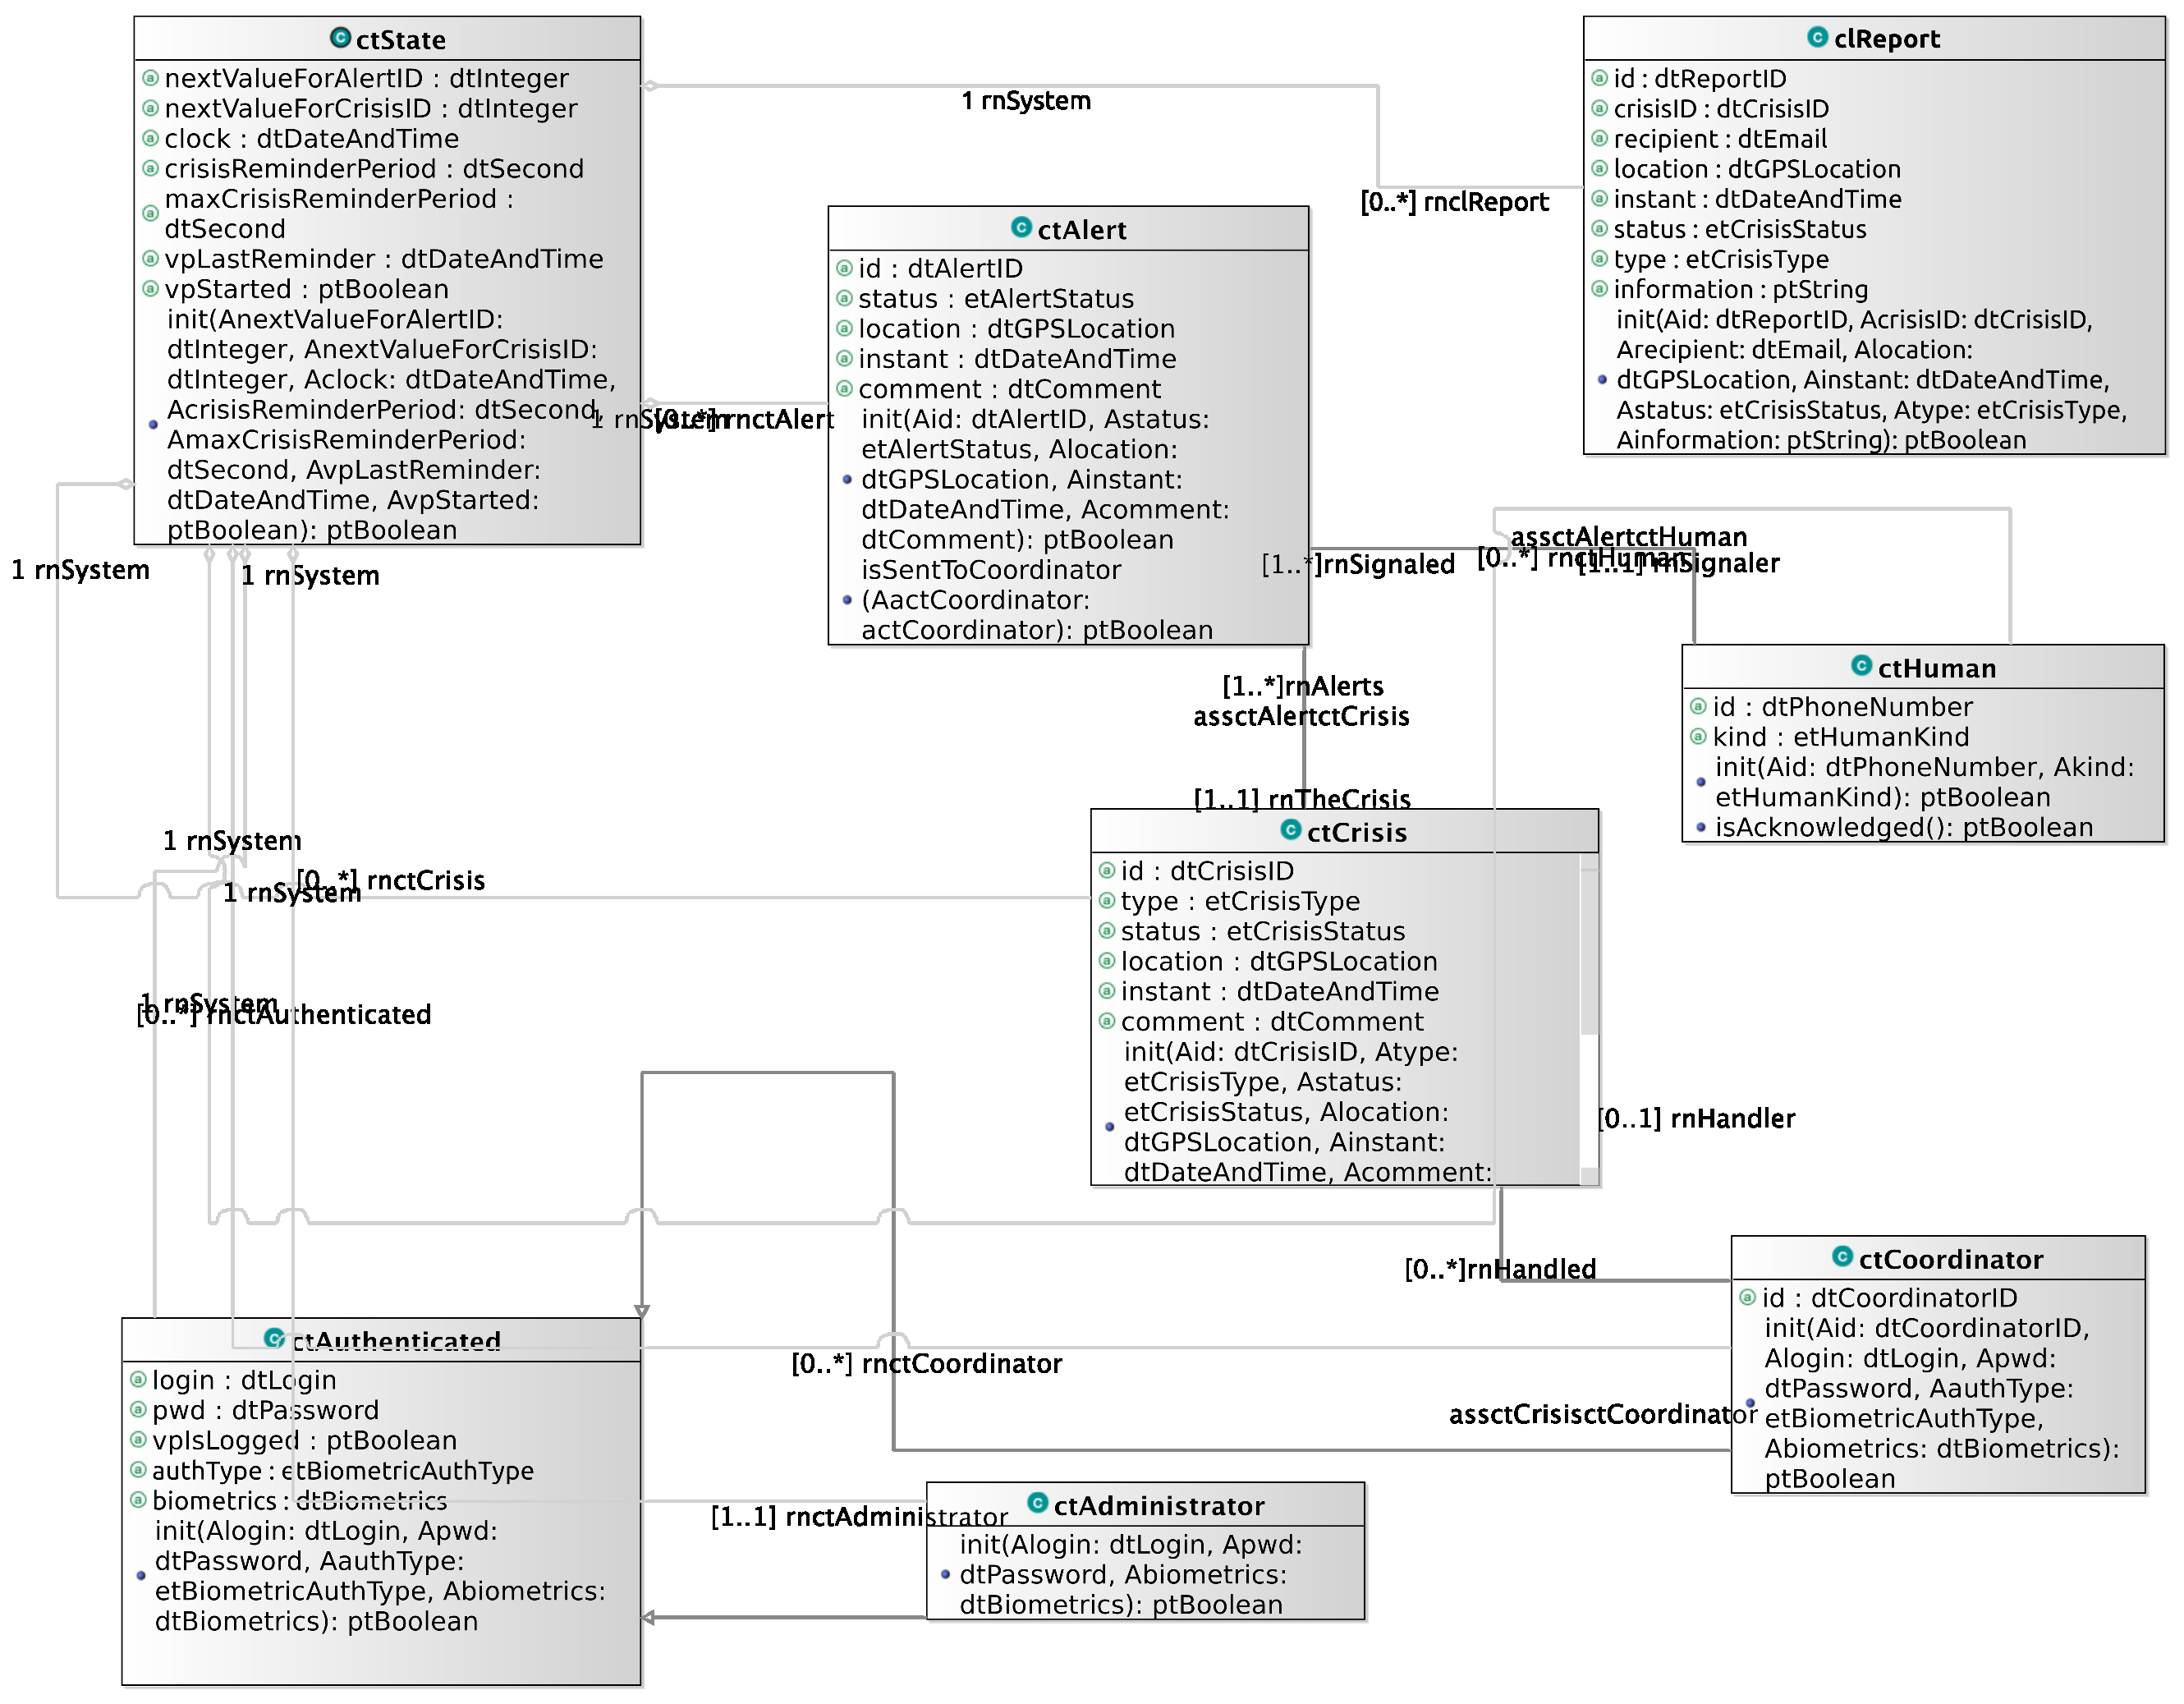
\includegraphics[width=\textwidth]{images/analysis/concept-model/global/PrimaryTypes-Classes/cm-pt-ct-lv-01-with-clReport.eps}
% 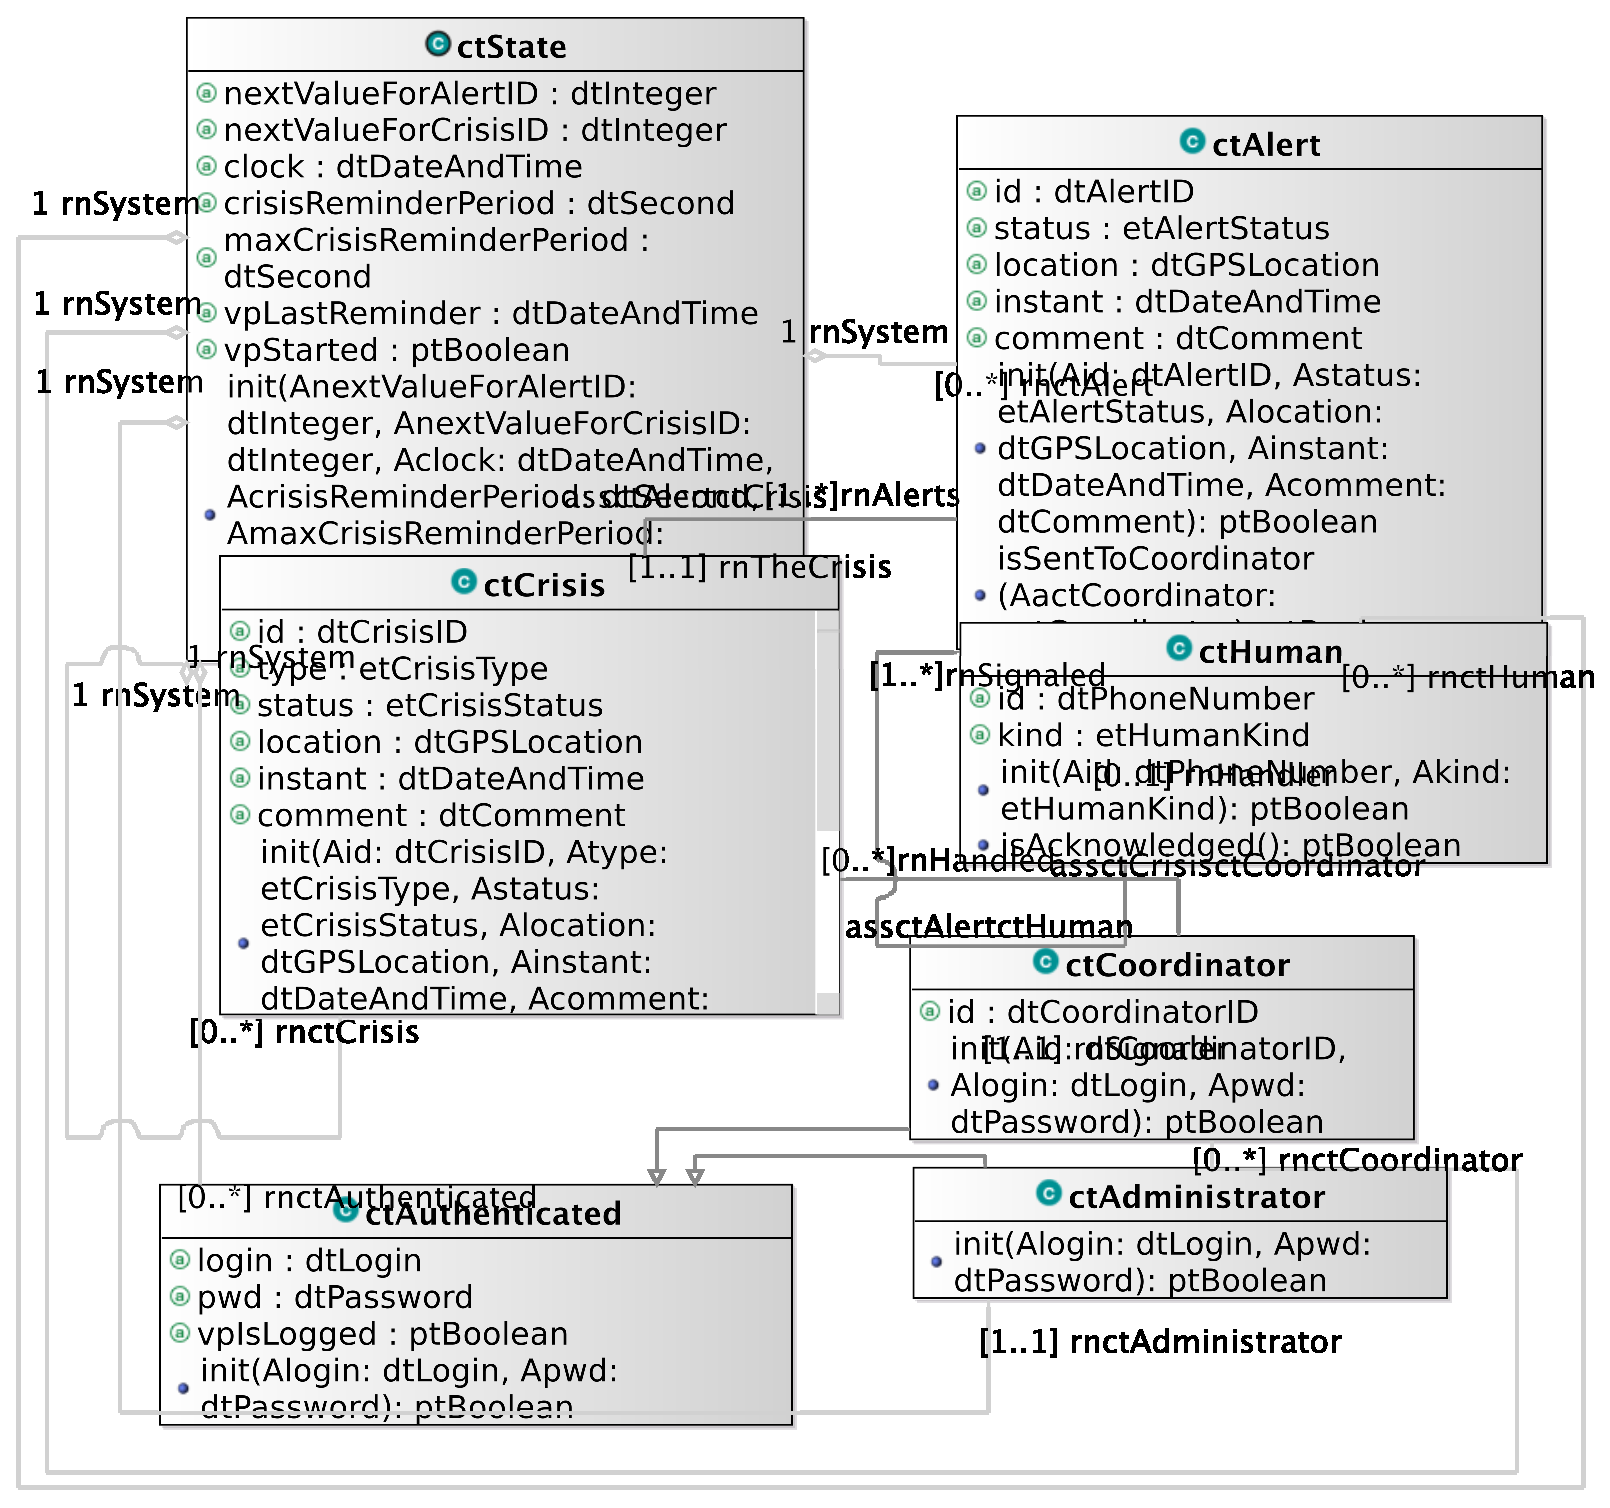
\includegraphics[width=\textwidth]{./images/analysis/01/global/cm-pt-ct-lv-01.eps}
%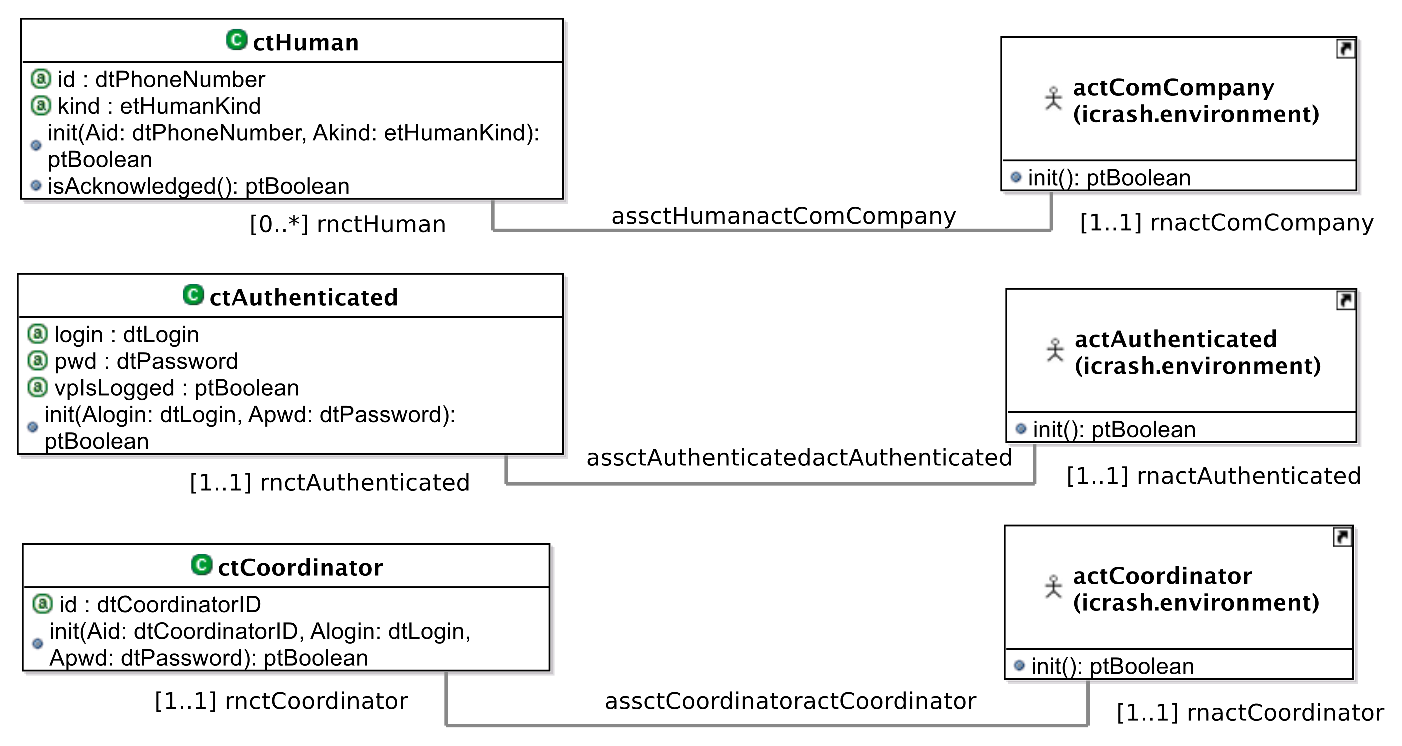
\includegraphics[width=\textwidth]{./images/analysis/concept-model/global/PrimaryTypes-Classes/01/cm-pt-ct-gv-01.eps}
\end{center}
\caption{Concept model - PrimaryTypes-Classes}
\label{fig:conceptClasses}
\end{figure}


\begin{itemize}

  	\item \textbf{ctAdministrator}
	Used to caracterize internally the entity that is responsible of administrating
	the \msricrash system.
	
	\item \textbf{ctAlert}
	Used to model crisis alerts sent by any human having communication capability
	using communication companies belonging to the system’s environment.
	
	\item \textbf{ctAuthenticated}
	Used to model system’s representation about actors that need to authenticate to
	access some specific functionalities.
	
	\item \textbf{ctCoordinator}
	Used to model system’s representation about the actors that have
	the responsibility to handle alerts and crisis.
	
	\item \textbf{ctCrisis} 
	Used to model crisis that are infered from the reception of at least
	one alert message. Crisis aer entities that are handled by the \msricrash system.
	
	\item \textbf{ctHuman} 
	Used to model system’s representation about the indirect actors that has
	alerted of potential crisis.
		
	\item \textbf{clReport}
	Used to model a report of the occurred crisis. 	It shows current state of the 
	accident to send the information to appropriate organizations.
	
	\item \textbf{ctState} 
	Used to model the system. There is only one instance at any state of the
	abstract machine after creation.

\end{itemize}

\subsection{Primary types - Datatypes types descriptions}

The diagram \ref{fig:conceptDataTypes} shows the basic data types of the
\msricrash system primary datatypes.

\begin{figure}[H]
\begin{center}
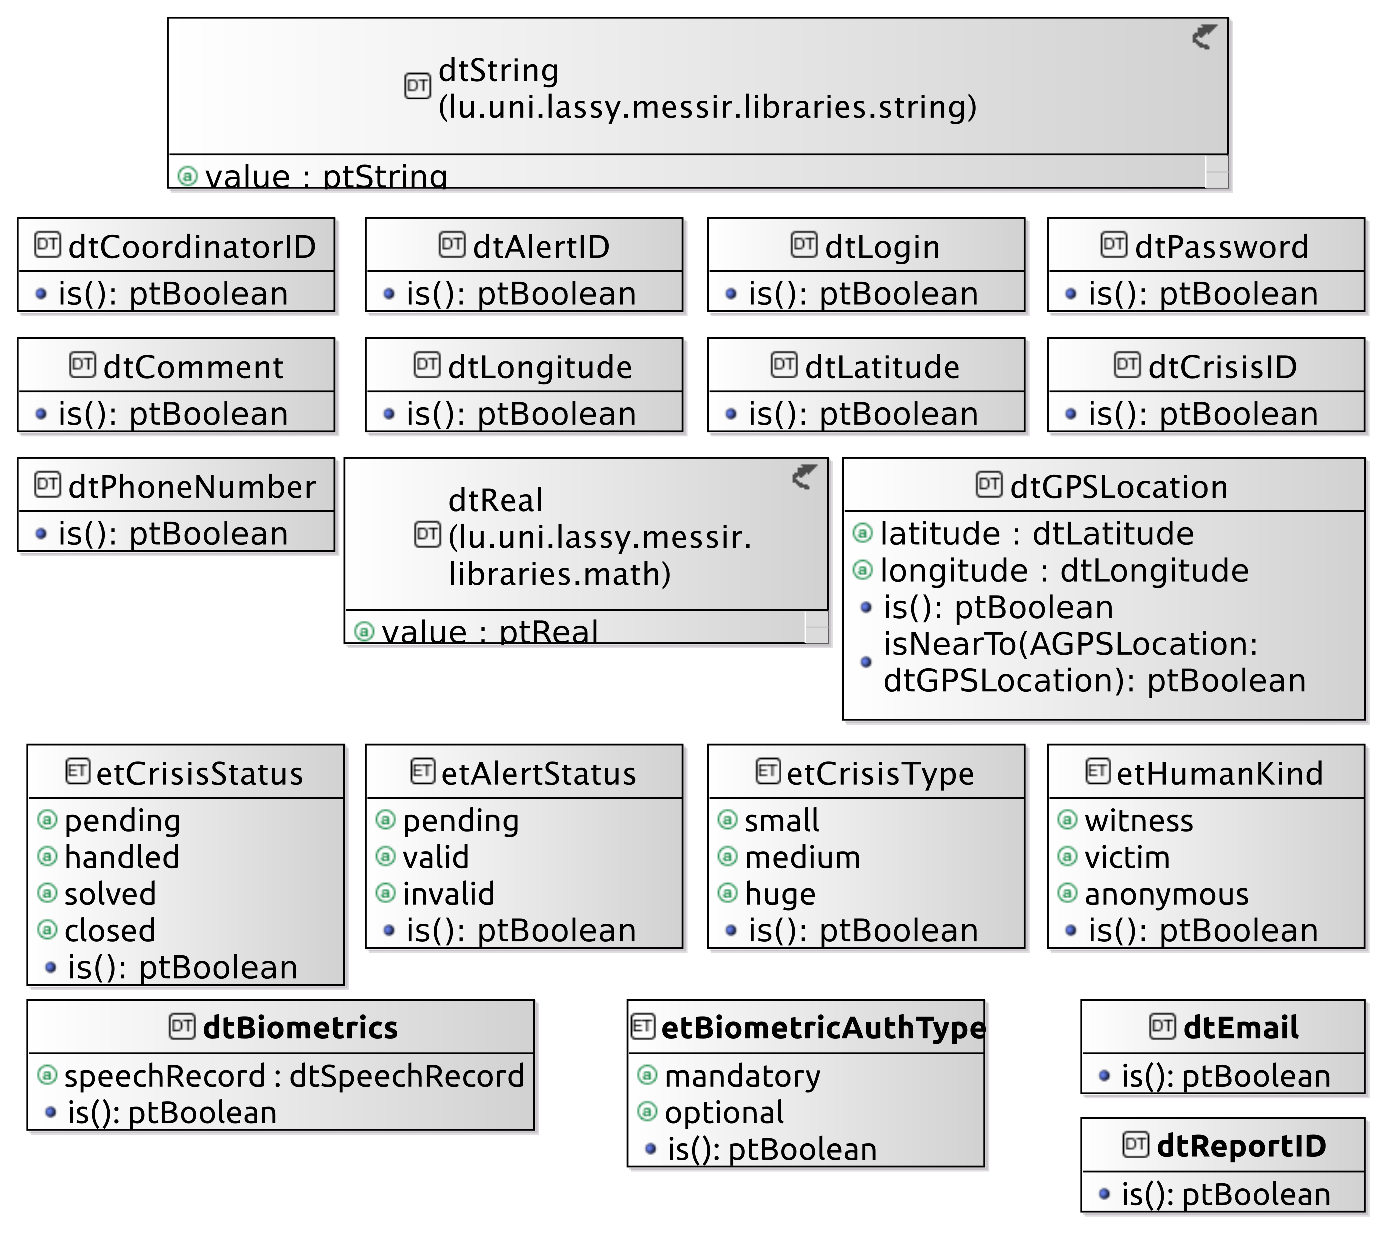
\includegraphics[width=\textwidth]{images/analysis/concept-model/global/PrimaryTypes-Classes/cm-pt-dt-gv-01.eps}
\end{center}
\caption{Concept model - PrimaryTypes-Classes}
\label{fig:conceptDataTypes}
\end{figure}

\subsubsection{Datatypes}
\begin{itemize}
	\item \textbf{dtAlertID}
	A string used to identify alerts.
	
	\item \textbf{dtComment}
	A datatype made of a string value used to receive,store and send
	textual information about crisis and alerts.
	
	\item \textbf{dtCoordinatorID}
	A string used to identify coordinators.
	
	\item \textbf{dtCrisisID}
	A string used to identify crisis.
	
	\item \textbf{dtGPSLocation}
	Used to define coordinates of geograpical positions on earth. It
	is defined a couple made of a latitude and a longitude.
	
	\item \textbf{dtLatitude}
	Used to define a latitude value of a geograpical positions on earth.
	
	\item \textbf{dtLogin}
	A login string used to authentify an \msricrash user
	
	\item \textbf{dtLongitude}
	Used to define a longitude value of a geograpical positions on
	earth.
	
	\item \textbf{dtPassword}
	A password string used to authentify an \msricrash user
	
	\item \textbf{dtPhoneNumber}
	A string used to store the phone number from the human declaring
	the crisis or the alert.
	
	\item \textbf{dtEmail}
	A string used to store the email address of the recipient of the crisis
	report.
	
	\item \textbf{ReportID}
	A string used to identify reports.
\end{itemize}
\subsubsection{Enumerations}

\begin{itemize}
	\item \textbf{etAlertStatus}
	This type is used to indicate the different validation status of
	an alert.
	
	\item \textbf{etCrisisStatus}
	This type is used to indicate the different handling status of a
	crisis.
	
	\item \textbf{etCrisisType} 
	This type is used to indicate the different types of a crisis.
	
	\item \textbf{etHumanKind} 
	This type is used to indicate the kind of human that informs about a
	car crash crisis.
	
	\item \textbf{etBiometricAuthType}
	This type is used to indicate the different possibilities of biometric
	authentication.
\end{itemize}

\subsection{Secondary types - Datatypes types descriptions}

\subsubsection{Datatypes}
\begin{itemize}
  \item \textbf{dtSMS}
A datatype made of a string value used to send textual information to human
mobile devices. 
  \item \textbf{dtSpeechRecord}
  A datatype made of a record value used to determine human's voice 
\end{itemize}


   

\section{Environment Model}

The diagram \ref{fig:environmentGlobal} shows a global view of the \msricrash
system environment model.

\begin{figure}[H]
\begin{center}
  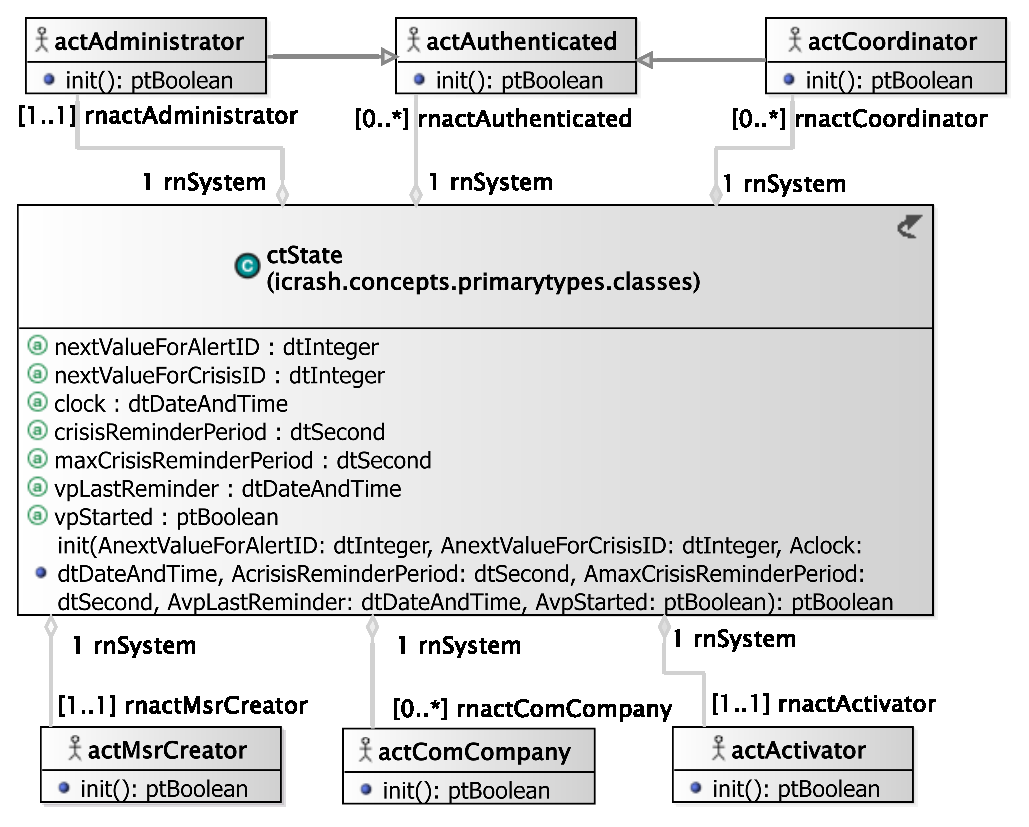
\includegraphics[width=400px]{images/analysis/environment-model/global/em-gv-01.eps}
  \caption{Environment Model - Global View}
  \label{fig:environmentGlobal}
\end{center}
\end{figure}

\begin{itemize}
	\item \textbf{actActivator Actor}
	Represents a logical actor for time automatic message sending based on system’s
	or environment status.
	
	\item \textbf{actAdministrator Actor}
	Represents an actor responsible of administration tasks for the \msricrash
	system. 
	
	\item \textbf{actAuthenticated Actor}
	Abstract actor providing reusable input and output interfaces for actors that
	need to authenticate themselves.
	
	\item \textbf{actComCompany Actor}
	Represents the communication company stakeholder ensuring the input/ouput of
	textual messages with humans having communication devices.
	
	\item \textbf{actCoordinator Actor}
	Represents actor responsible of handling one or several crisis for the
	\msricrash system.
	
	\item \textbf{actMsrCreator Actor}
	Represents the creator stakeholder in charge of state and environment
	initialization.

\end{itemize}

